\chapter{Displaced tracking efficiency}
\label{displaced_tracking_eff}
To measure the efficiency to reconstruct displaced, isolated, high-\pt muons, our collaborator Ian Tomalin performed a study with cosmic rays. The basic idea is to approximate the displaced tracking efficiency in data and simulation from the fraction of cosmic-ray muons reconstructed in the muon system that have a corresponding track in the tracker. The results of this study are used to assign a systematic uncertainty in the signal efficiency (see Section~\ref{systematics}) and define the upper bound of \SI{10}{\cm} on the inclusive signal region (see Section~\ref{selection}).

First, the cosmic-ray dataset is chosen. CMS collects cosmic-ray data in two types of runs: (1) dedicated cosmic runs in which cosmic-ray muons are reconstructed with dedicated reconstruction algorithms and (2) parasitic cosmic runs in which the triggers veto bunch-crossing events to collect cosmic-ray data in otherwise normal proton-proton running conditions. In the parasitic cosmic runs, the cosmic-ray muons are reconstructed with the standard reconstruction algorithms as well as some dedicated reconstruction algorithms. These two types of runs are then collected into two datasets: (1) \texttt{Cosmics}, which contains only the dedicated cosmic runs and (2) \texttt{NoBPTX}, which contains both the dedicated and parasitic cosmic runs. In each case, the strip tracker electronics operate in the same mode used for proton-proton collisions. The \texttt{NoBPTX} datasets are used in this study because they include the same reconstruction algorithms as used in the Displaced Leptons analysis.

Events are collected with the \longvar{HLTL2Mu10NoVertexNoBPTX3BXv*} trigger, which vetoes events with proton-proton collisions and requires that a muon with $\pt>\SI{10}{\GeV}$ is reconstructed in the muon system. As in the Displaced Leptons analysis, the trigger does not explicitly constrain the muon $d_0$ or $d_z$. Following the study presented in Appendix~\ref{k0}, only eras G and H are used in 2016. The set of data-taking periods with reliable detector performance is identified with particular attention paid to the following properties: (1) suitable cosmic trigger timing configuration, (2) data quality assessed from reconstructed (as opposed to trigger-level) quantities, (3) trigger, tracker, muon system, and track reconstruction known to be functioning well, and (4) magnetic field value in normal range.

To compare the displaced tracking efficiency between data and simulation, simulated cosmic-ray events are produced using the CMSCGEN generator~\cite{cmscgen}. The simulated cosmic-ray muons have $\pt>\SI{20}{\GeV}$, $\ad<\SI{40}{\cm}$, $\abs{d_z}<\SI{80}{\cm}$, and arrive within a \SI{30}{\ns} window centered on the time at which tracker readout efficiency is greatest. The detector response is modeled with GEANT~\cite{geant4}.

In both data and simulated events, cosmic rays are reconstructed in the tracker using the same track reconstruction algorithm that is used during proton-proton collisions. This algorithm assumes particles propagate outwards from the center of the detector, so cosmic-ray muons are typically reconstructed as two tracks: one moving upward and one moving downwards. In the muon system, cosmic-ray muons are reconstructed with two dedicated algorithms. The first is a two-leg algorithm that reconstructs each cosmic-ray muon as two separate muons, one in the top half of CMS and the other in the bottom. The second is a one-leg algorithm that reconstructs cosmic rays as a single muon that traverses the entire detector. The longer lever arm provided by the one-leg algorithm generally results in more accurate measurements of the muon curvature in the magnetic field.

A preliminary event selection is then applied to the data and simulation. The events are required to have one one-leg muon with $\pt>\SI{20}{\GeV}$ and at least \num{50} hits in the muon system. While the \pt requirement of the muons selected in this study is lower than the Displaced Leptons muon \pt requirement, the tracking efficiency does not depend significantly on \pt in the relevant range. The one-leg muon is also required to be within \SI{0.3}{\radian} of two two-leg muons in $\phi$ in order to reject cosmic-ray muon candidates that do not traverse the entire detector.

The tracking efficiency is inferred from the fraction of selected one-leg muons that are associated with a tracker track that has $\pt>\SI{15}{\GeV}$ and is within \SI{0.2}{\radian} in $\phi$ of the selected one-leg muon. To mimic the Displaced Leptons event selection, tracker tracks are also required to have at least one pixel hit. Because each cosmic-ray muon generally results in two tracker tracks, two separate efficiencies are measured. These efficiencies are referred to as ``upward" and ``downward" according to the direction of the relevant tracker track. The downward efficiency is expected to be more reliable because the tracker readout electronics assume that particles propagate outward from the center of the detector. The upward and downward efficiencies measured in this study agree within a few percent, but the downward efficiencies are used for the definitive measurement.

The muon system also measures the cosmic-ray muon arrival time. The average of the two two-leg muon arrival times provides the most precise measurement of the cosmic-ray muon arrival time. This approach provides a time resolution on the order of \SI{5}{\ns}, whereas the time resolution provided by one-leg muons can be an order of magnitude greater.

The selected one-leg muons with $\ad<\SI{8}{\cm}$ and $\abs{d_z}<\SI{20}{\cm}$ are used to study the tracking efficiency dependence on cosmic-ray muon arrival time. Figure~\ref{arrival_time} shows the distribution of the measured arrival time while Fig.~\ref{trk_eff_vs_arrival_time} shows the measured downward tracking efficiency as a function of measured arrival time. The disagreement between data and simulation in measured arrival time is simply an artifact of the specified simulation time window. Despite this offset, the efficiency shows a clear peak with a width of approximately \SI{15}{\ns} in both data and simulation. Based on the results of Fig.~\ref{trk_eff_vs_arrival_time}, muons used in the downward tracking efficiency measurement must also pass the requirements listed in Table~\ref{arrival_time_requirements}. Using the upward efficiency produces similar results that are shifted by approximately \SI{5}{\ns}. The same sample of one-leg muons is also used to measure the downward tracking efficiency as a function of run number. No meaningful dependence is identified.

\begin{figure}
\centering
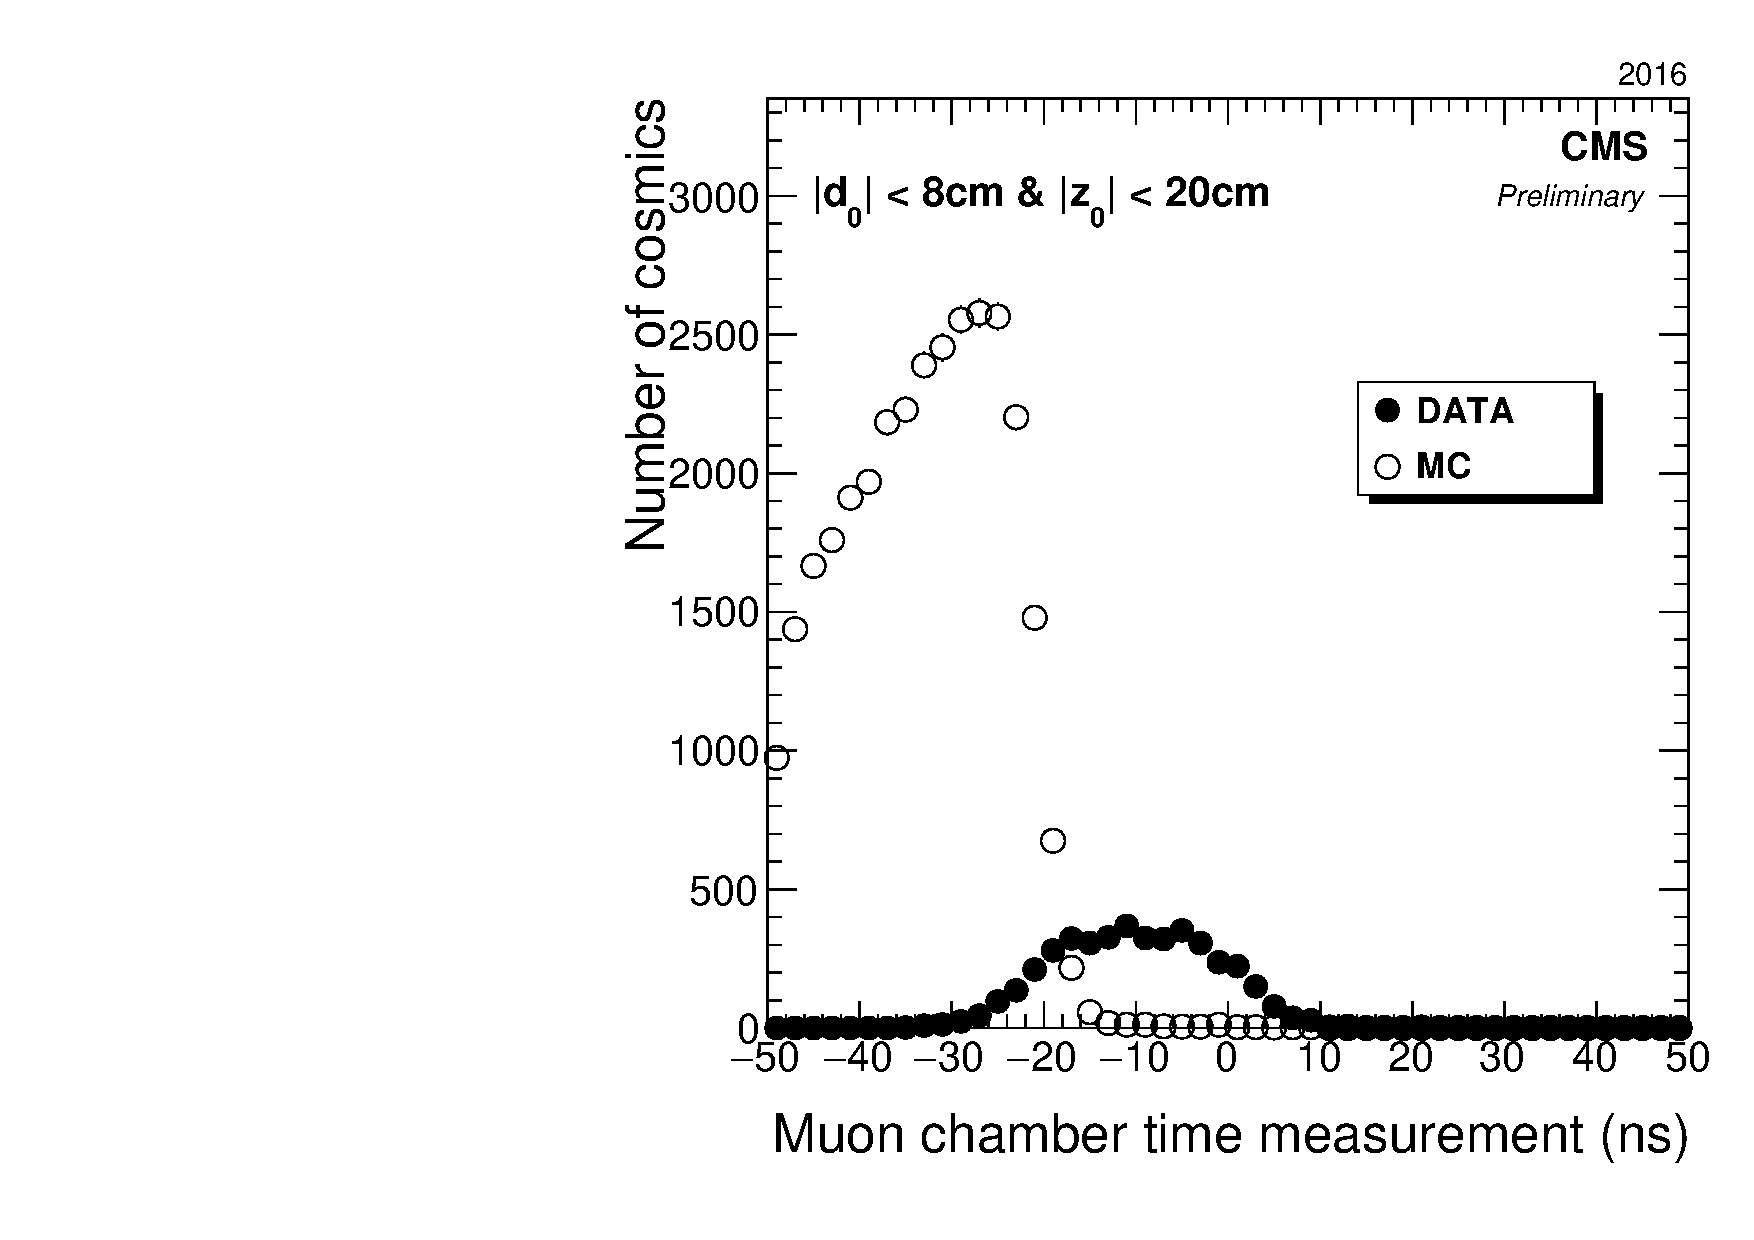
\includegraphics[width=0.4\textwidth]{figures/tracking_eff/2016/Muon2TimeAve.pdf}
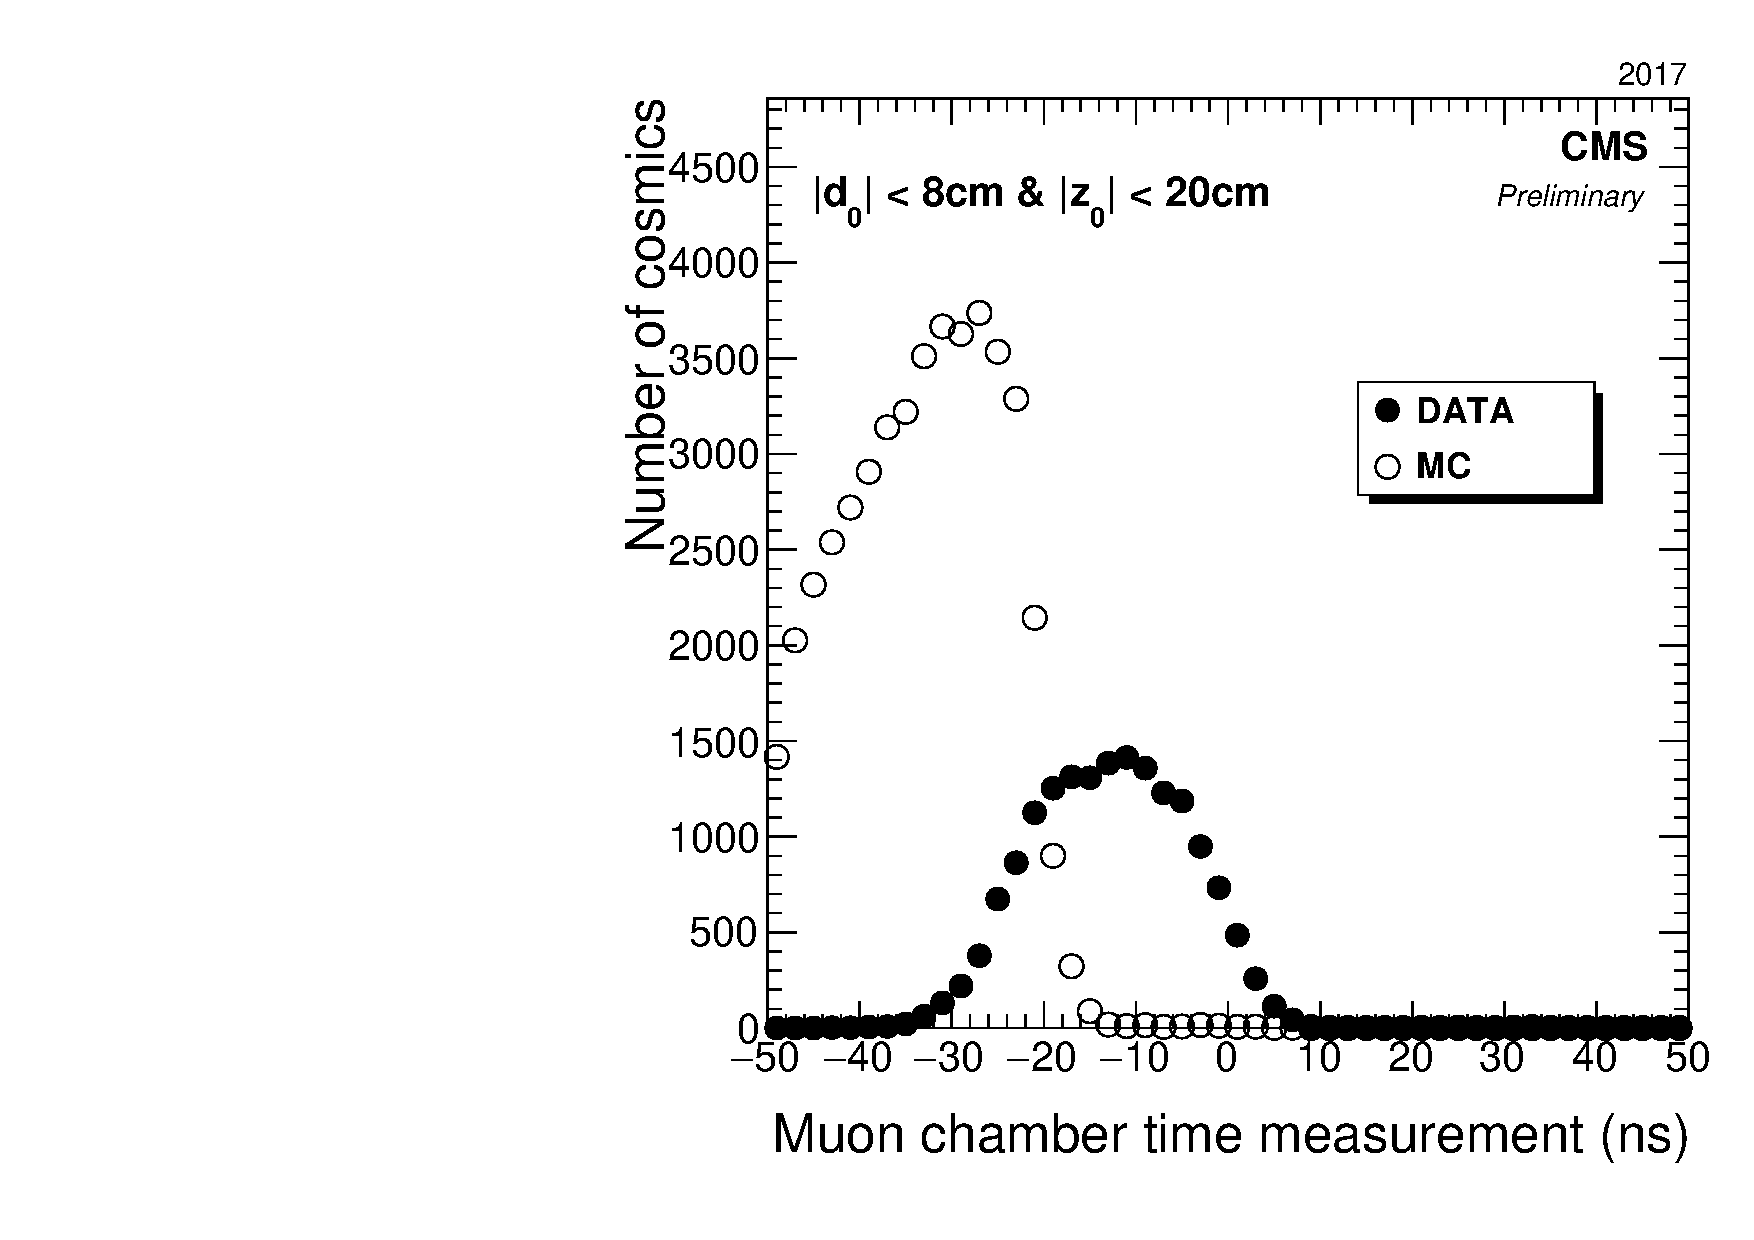
\includegraphics[width=0.4\textwidth]{figures/tracking_eff/2017/Muon2TimeAve.pdf}
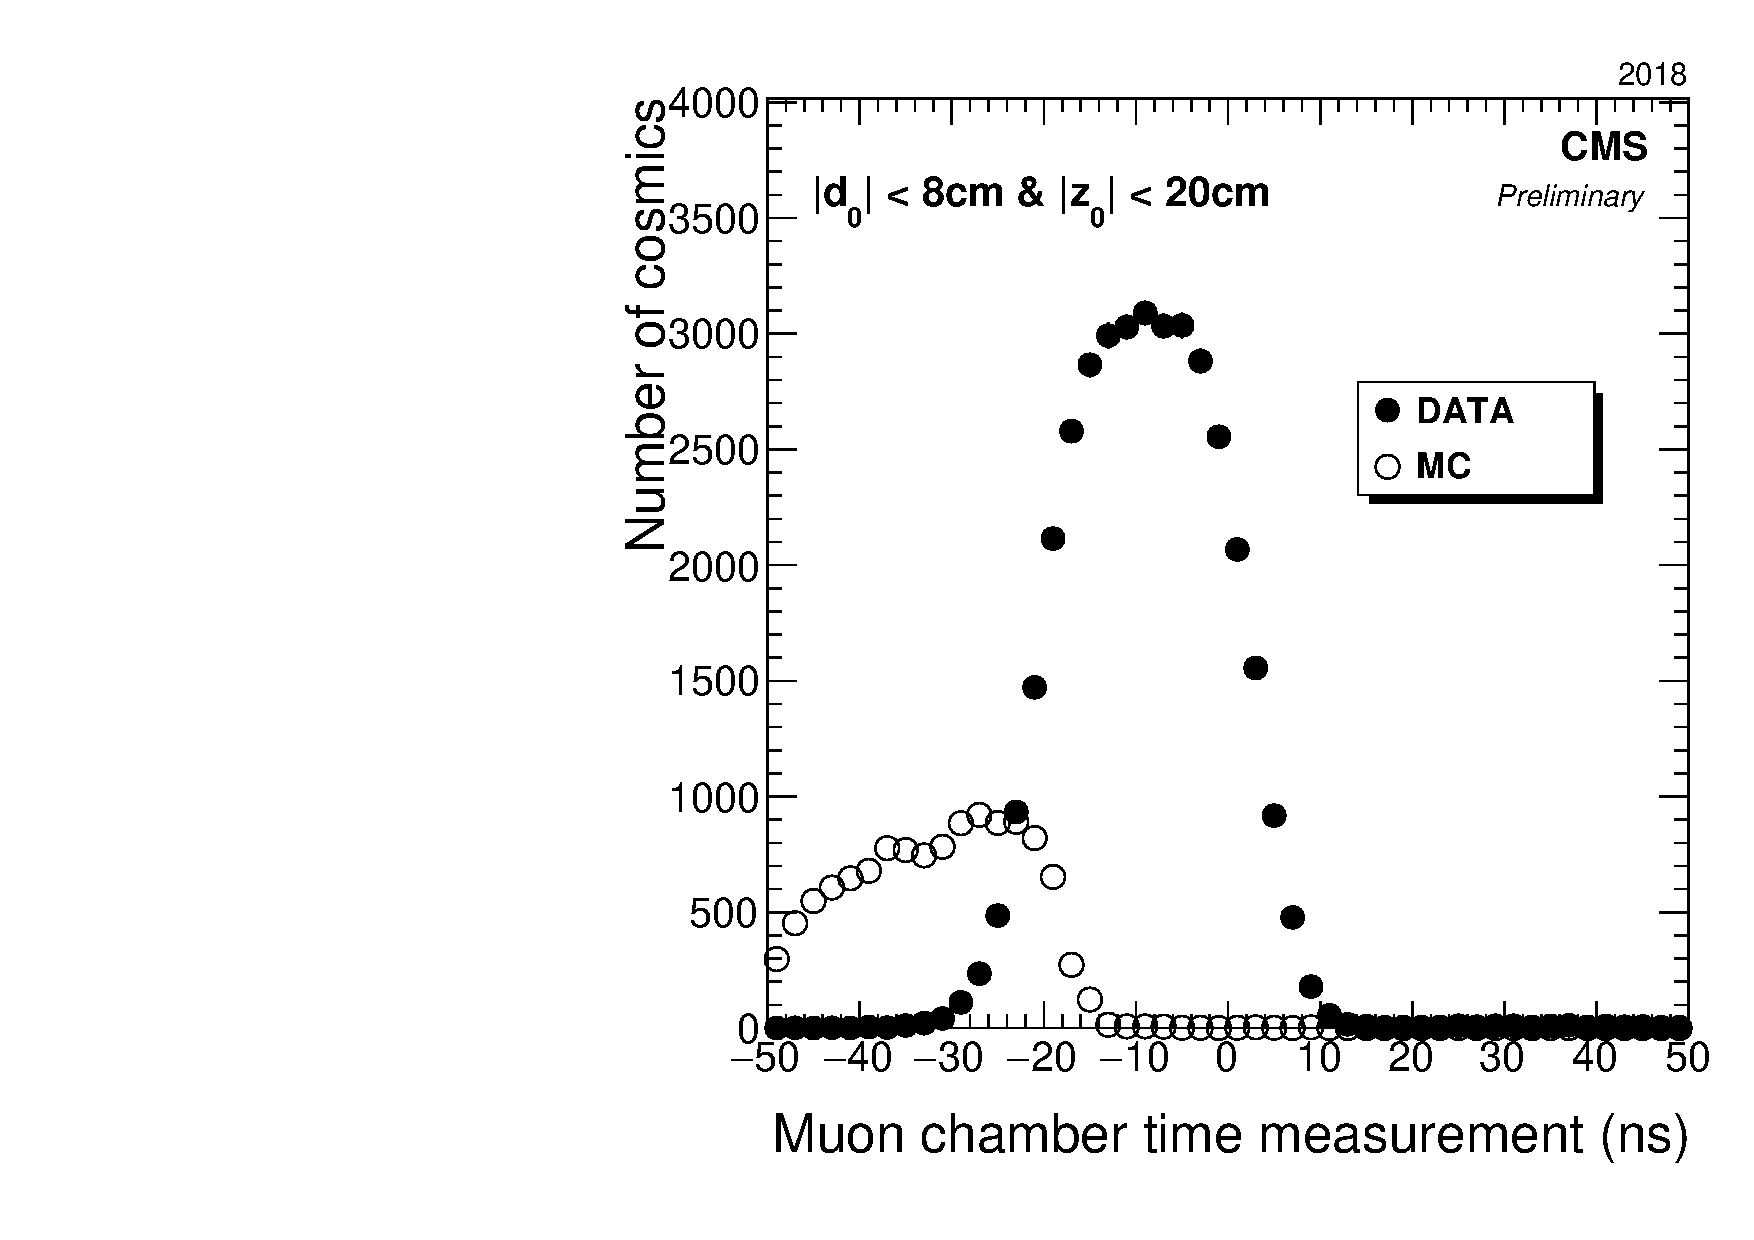
\includegraphics[width=0.4\textwidth]{figures/tracking_eff/2018/Muon2TimeAve.pdf}
\caption{Distribution of the arrival time of cosmic rays at their point of closest approach to the beamline as measured by the muon system in 2016 (top left), 2017 (top right), and 2018 (bottom) in data and simulation. Only cosmic ray muons with $\ad<\SI{8}{\cm}$ and $\az<\SI{20}{\cm}$ are considered.}
\label{arrival_time}
\end{figure}

\begin{figure}[hbtp]
\centering
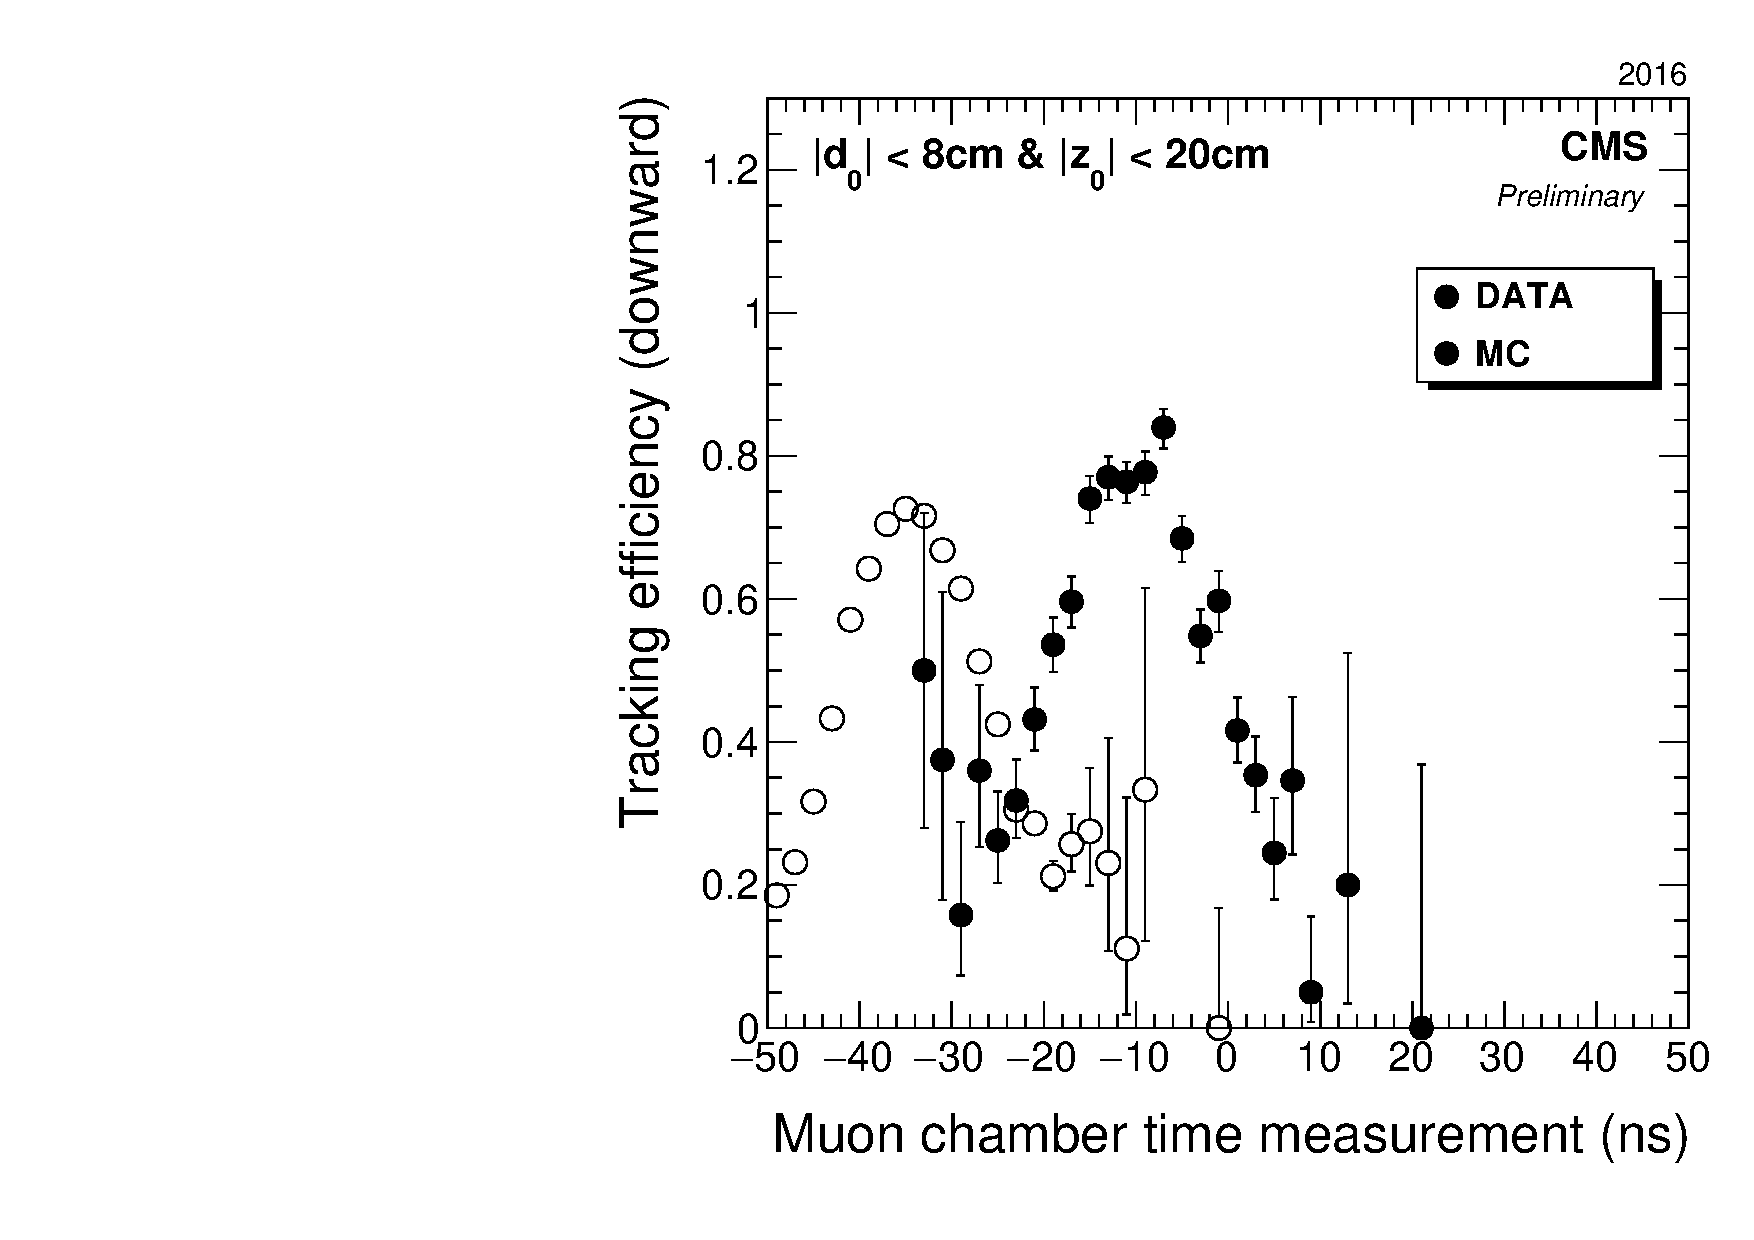
\includegraphics[width=0.4\textwidth]{figures/tracking_eff/2016/Eff0vsMuon2Time.pdf}
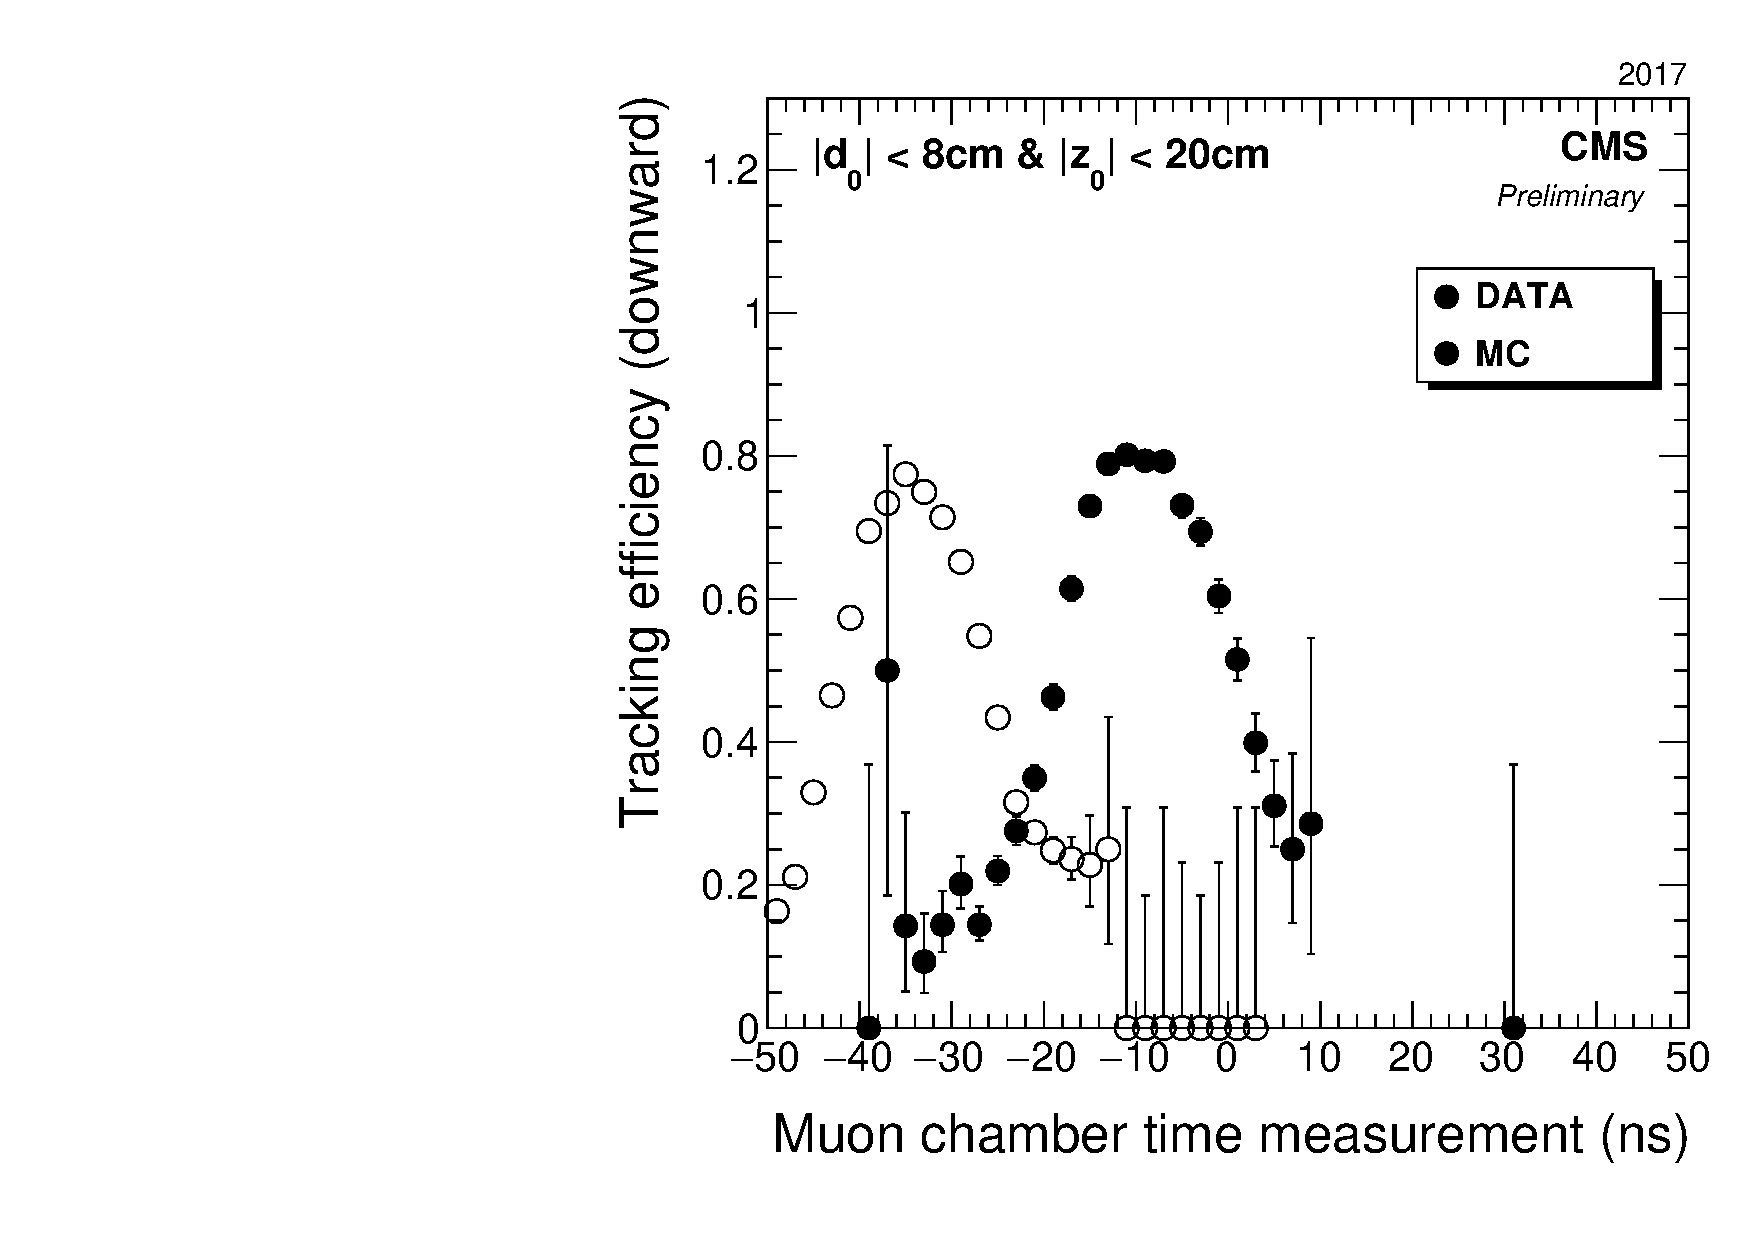
\includegraphics[width=0.4\textwidth]{figures/tracking_eff/2017/Eff0vsMuon2Time.pdf}
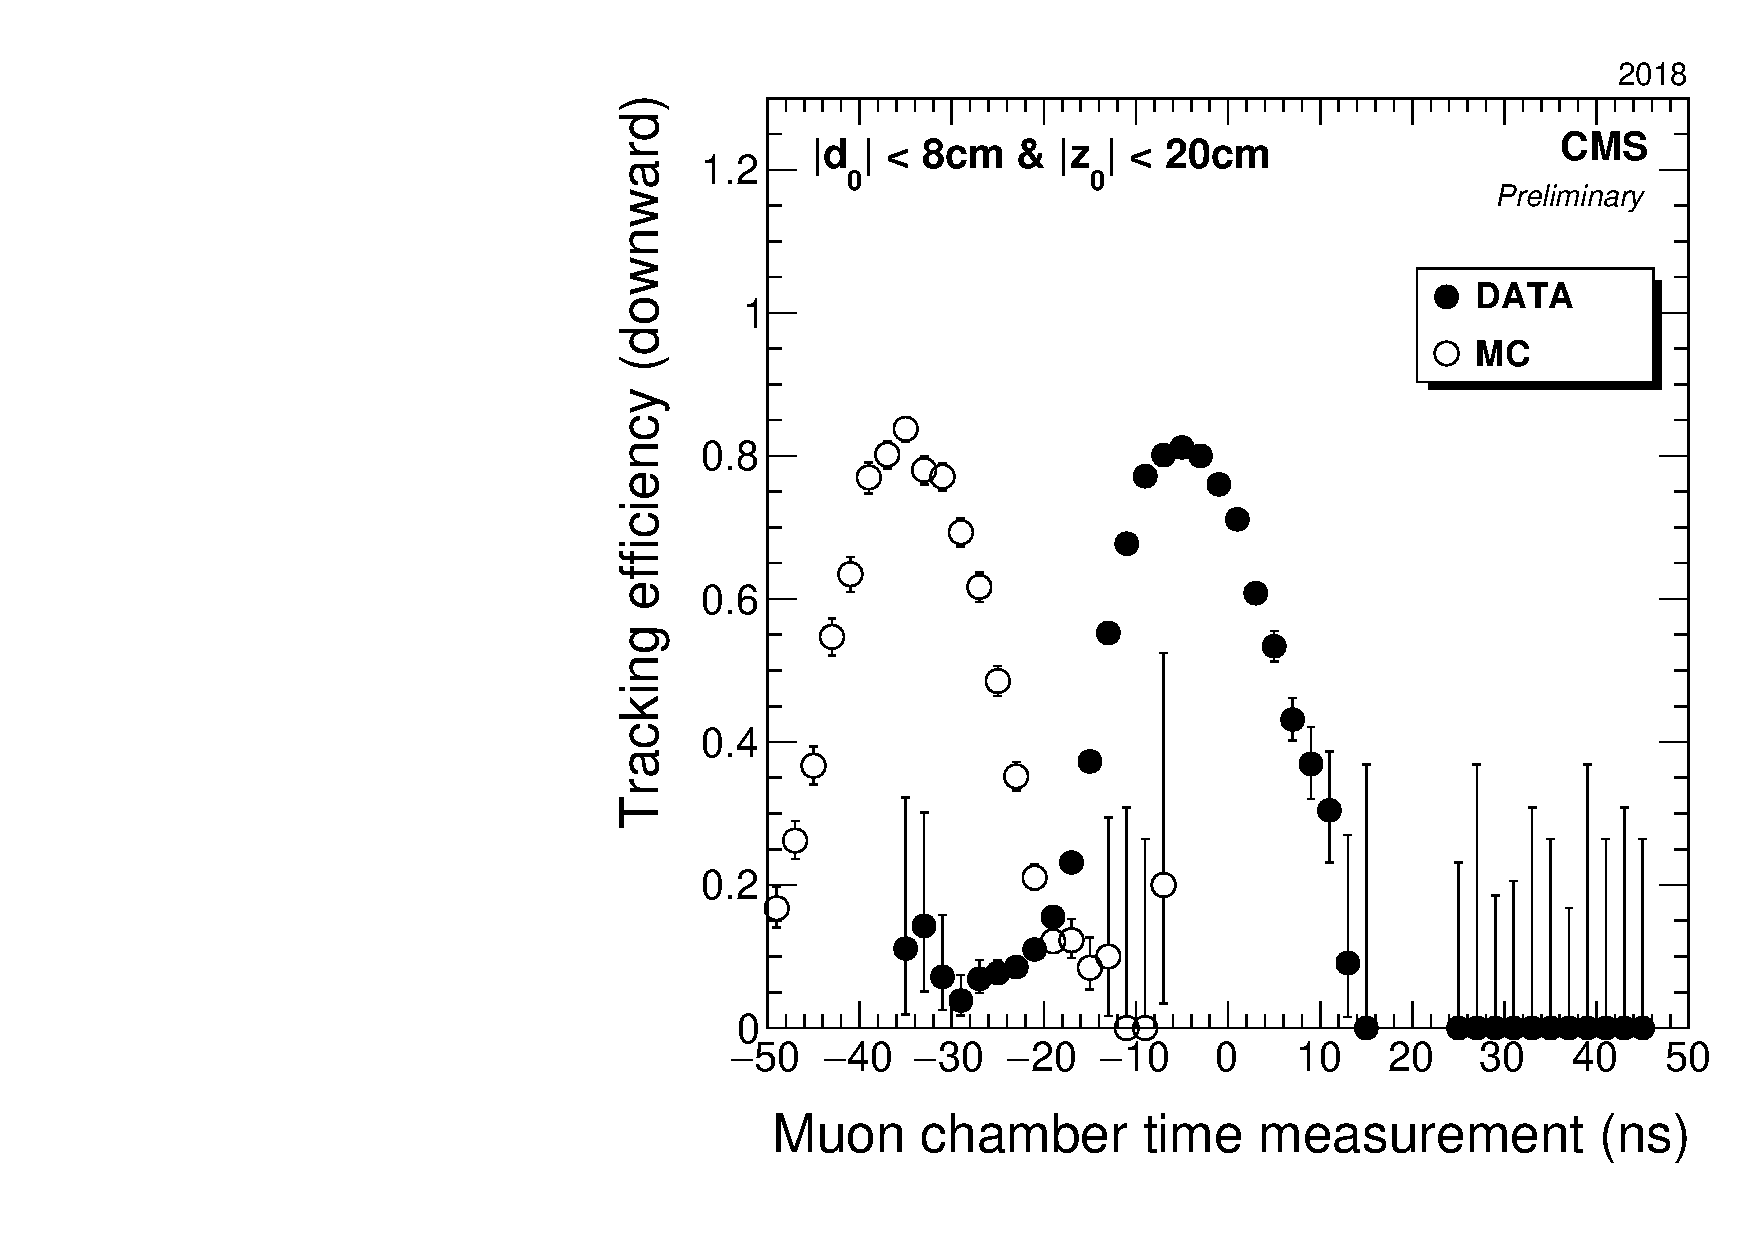
\includegraphics[width=0.4\textwidth]{figures/tracking_eff/2018/Eff0vsMuon2Time.pdf}
\caption{Measured downward tracking efficiency versus cosmic ray muon arrival time in 2016 (top left), 2017 (top right), and 2018 (bottom) in data and simulation. Only cosmic ray muons with $\ad<8$\cm and $\az<20$\cm are considered.}
\label{trk_eff_vs_arrival_time}
\end{figure}
\begin{table}
\noindent \centering{}
\topcaption{Cosmic ray muon arrival time requirements used when measuring displaced tracking efficiency in data and simulation.}
\label{arrival_time_requirements}
\begin{tabular}{l|cc}
\hline
           & 2016--2017                   & 2018\\
\hline
Data       & $\SI{-13}{\ns} < t_{muon} <  \SI{-7}{\ns}$ &  $\SI{-8}{\ns} < t_{muon} <  \SI{-2}{\ns}$\\
Simulation & $\SI{-38}{\ns} < t_{muon} < \SI{-32}{\ns}$ & $\SI{-40}{\ns} < t_{muon} < \SI{-34}{\ns}$\\
\hline
\end{tabular}
\end{table}

The downward tracking efficiency is then measured using all selected one-leg muons that meet the timing requirements specified in Table~\ref{arrival_time_requirements}. The downward tracking efficiency as a function of \ad and $\abs{d_z}$ is shown for all three years in Fig.~\ref{displaced_trk_eff_vs_d0dz}. The tracking efficiency is found to be nonzero out to at least $\ad\leq\SI{10}{\cm}$ and $\abs{d_z}\leq\SI{30}{\cm}$ in all three years. We also note that removing the pixel-hit requirement increases this range to approximately $\ad\leq\SI{30}{\cm}$ and $\abs{d_z}\leq\SI{50}{\cm}$.

\begin{figure}
\centering
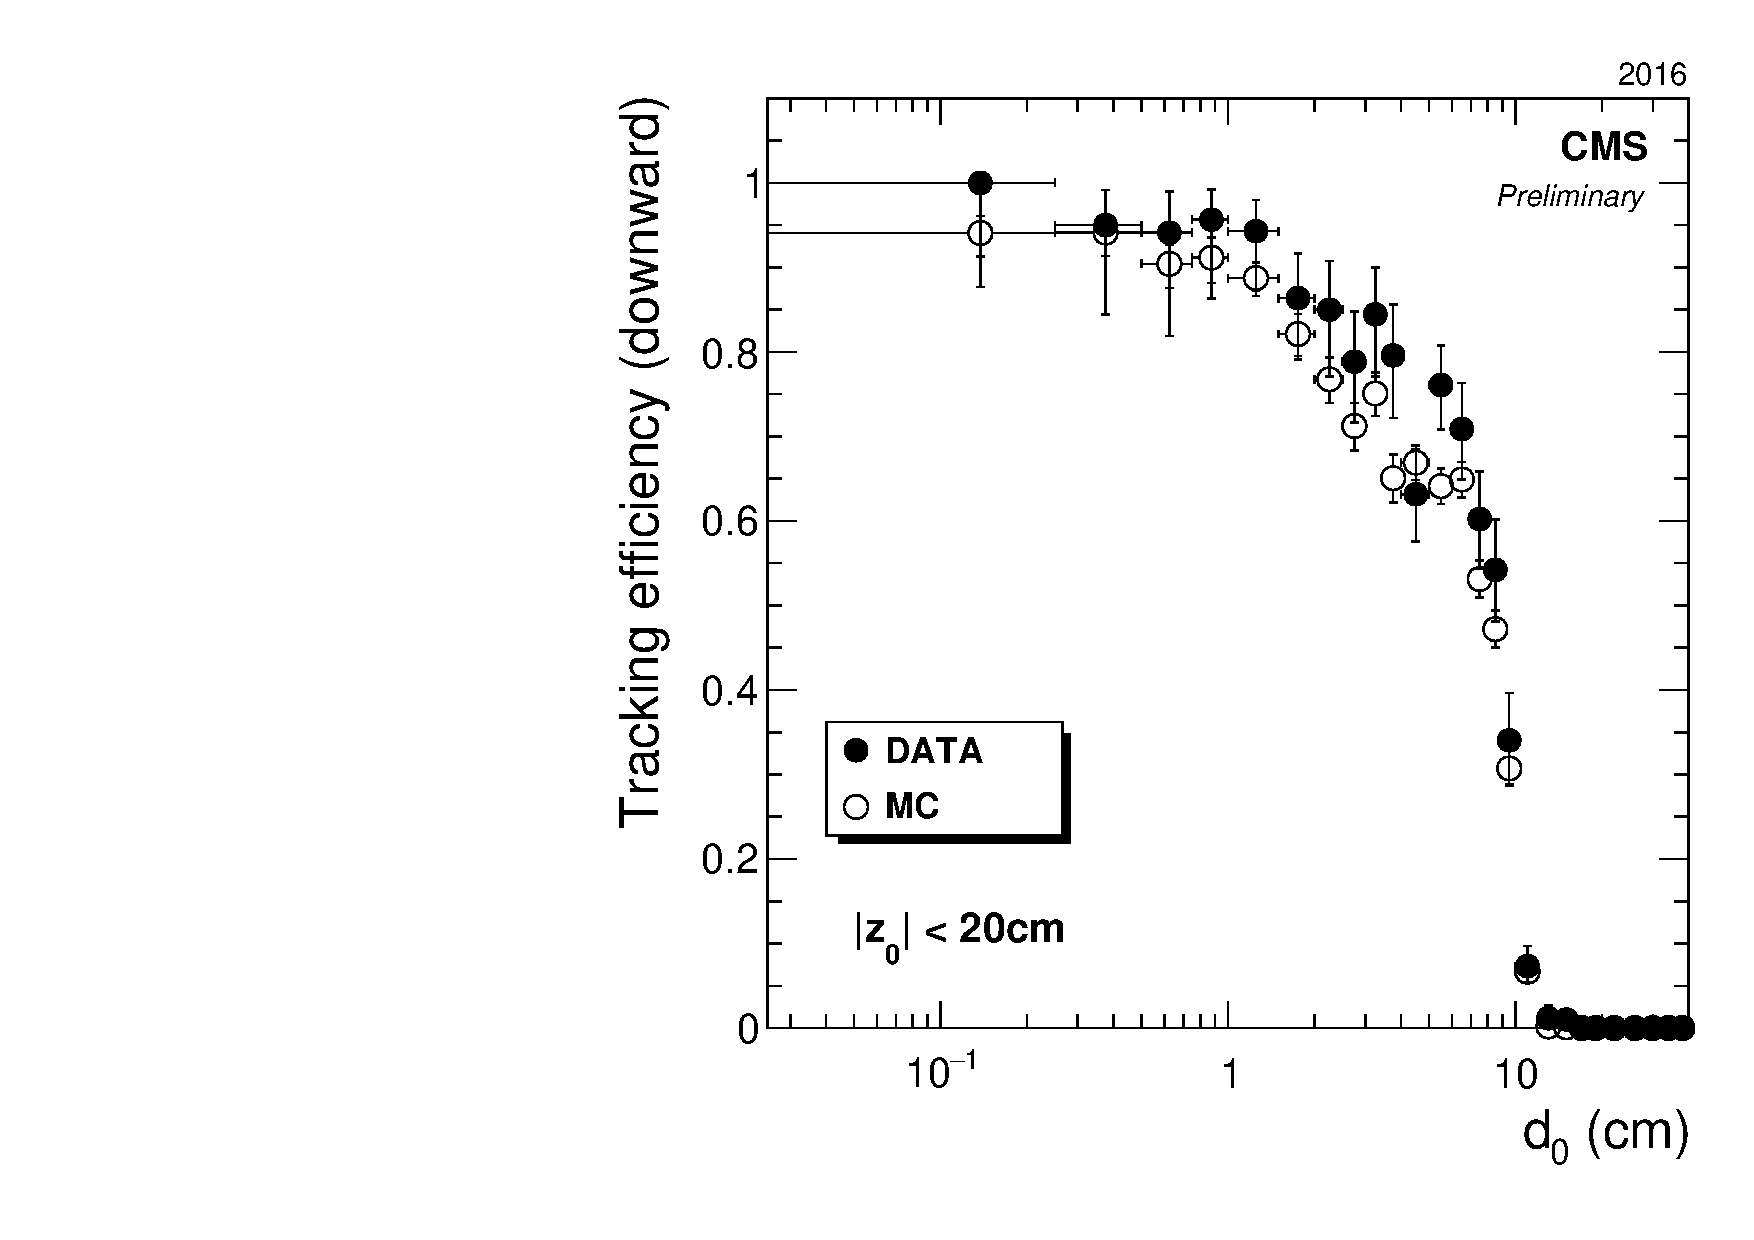
\includegraphics[width=0.4\textwidth]{figures/tracking_eff/2016/Eff0vsD0.pdf}
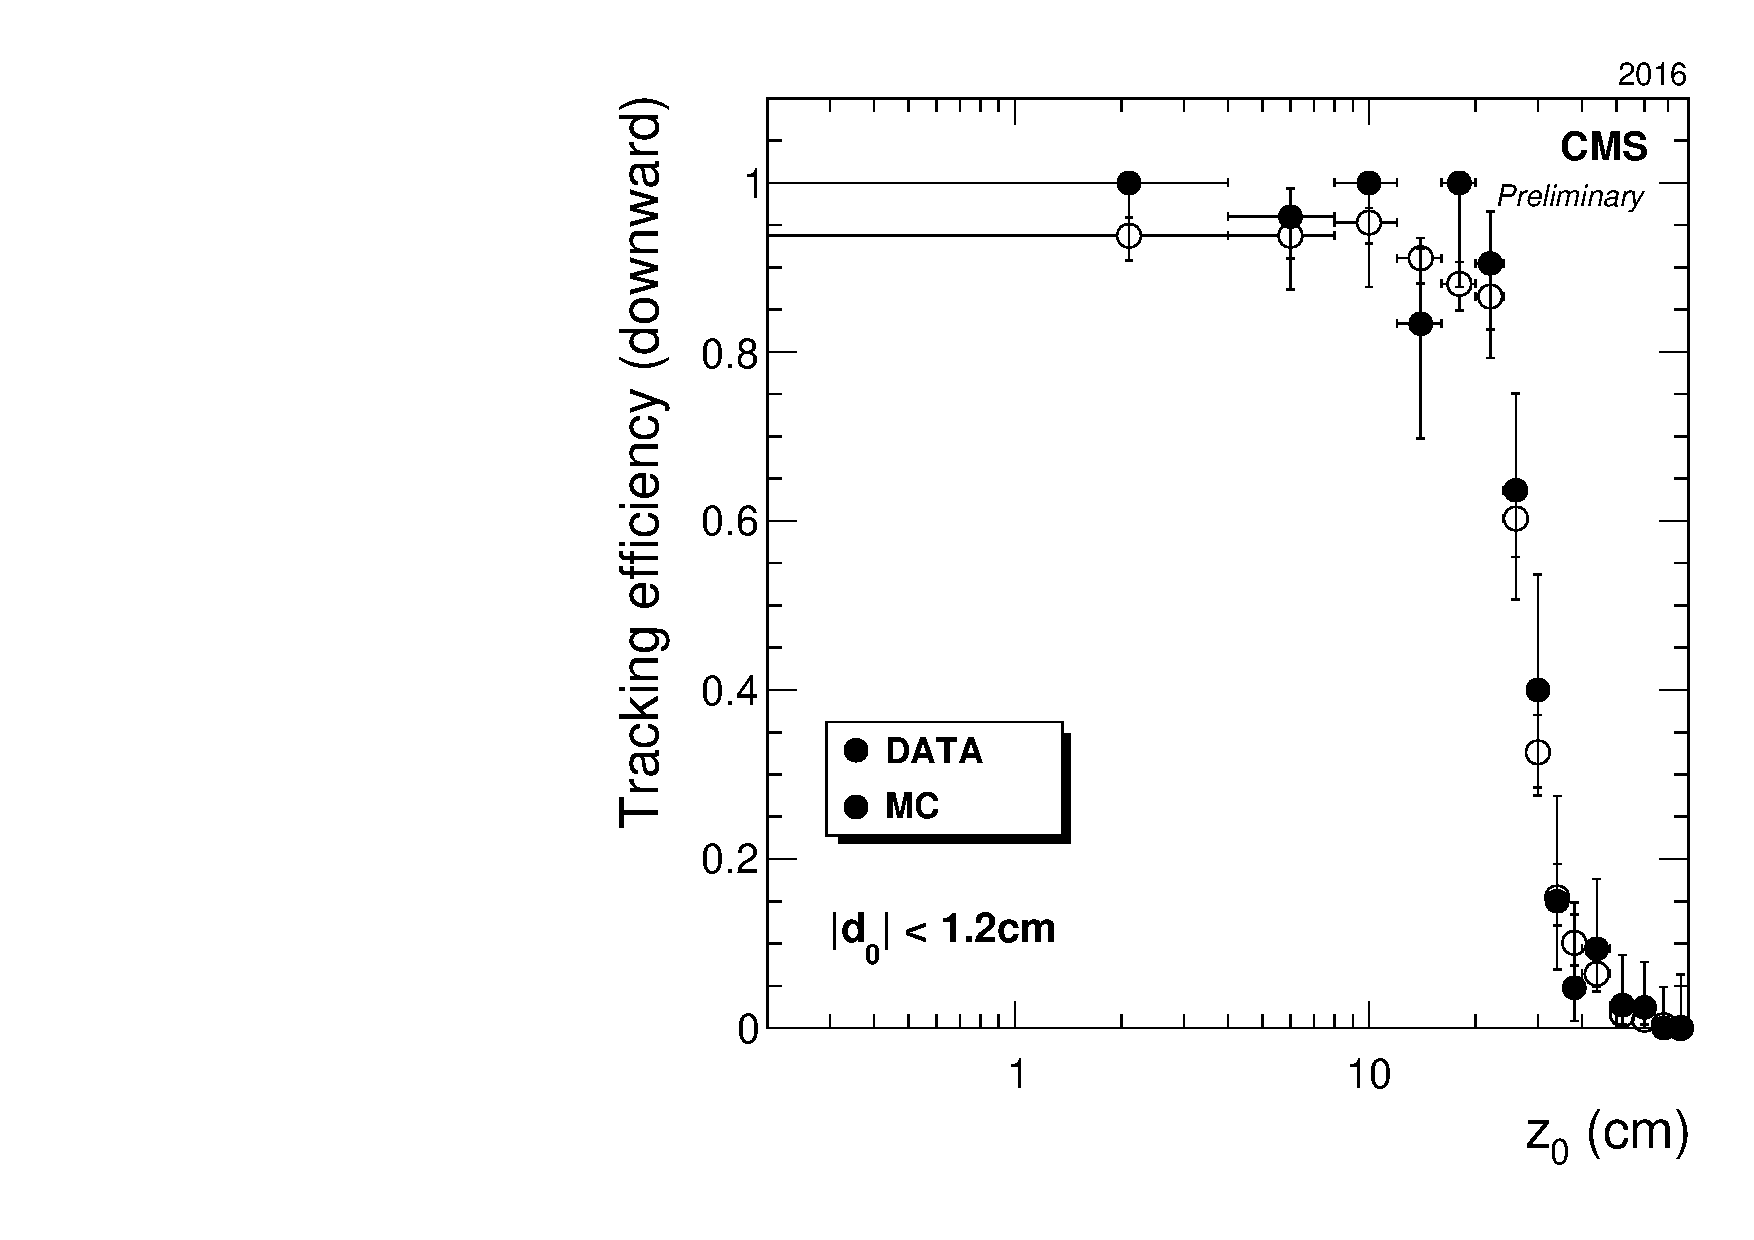
\includegraphics[width=0.4\textwidth]{figures/tracking_eff/2016/Eff0vsZ0.pdf}
\\
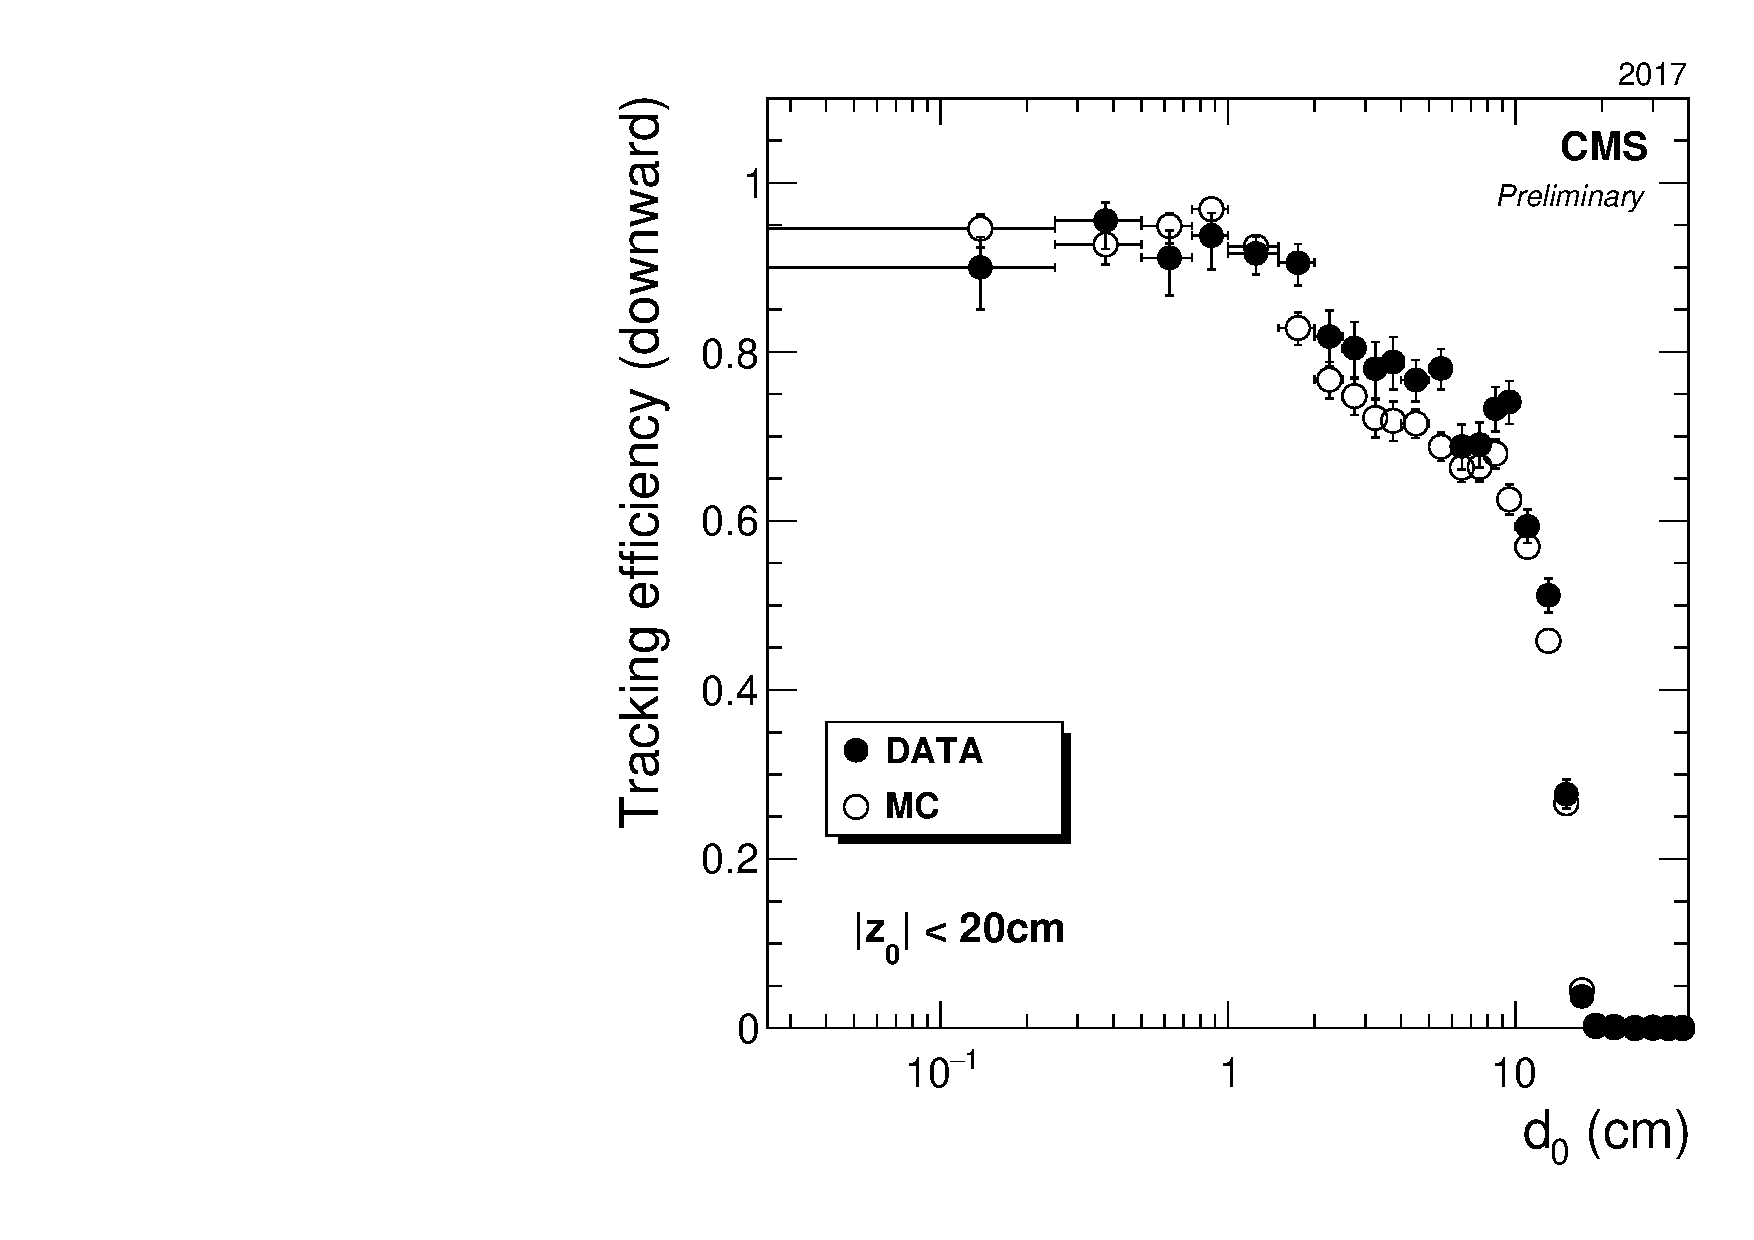
\includegraphics[width=0.4\textwidth]{figures/tracking_eff/2017/Eff0vsD0.pdf}
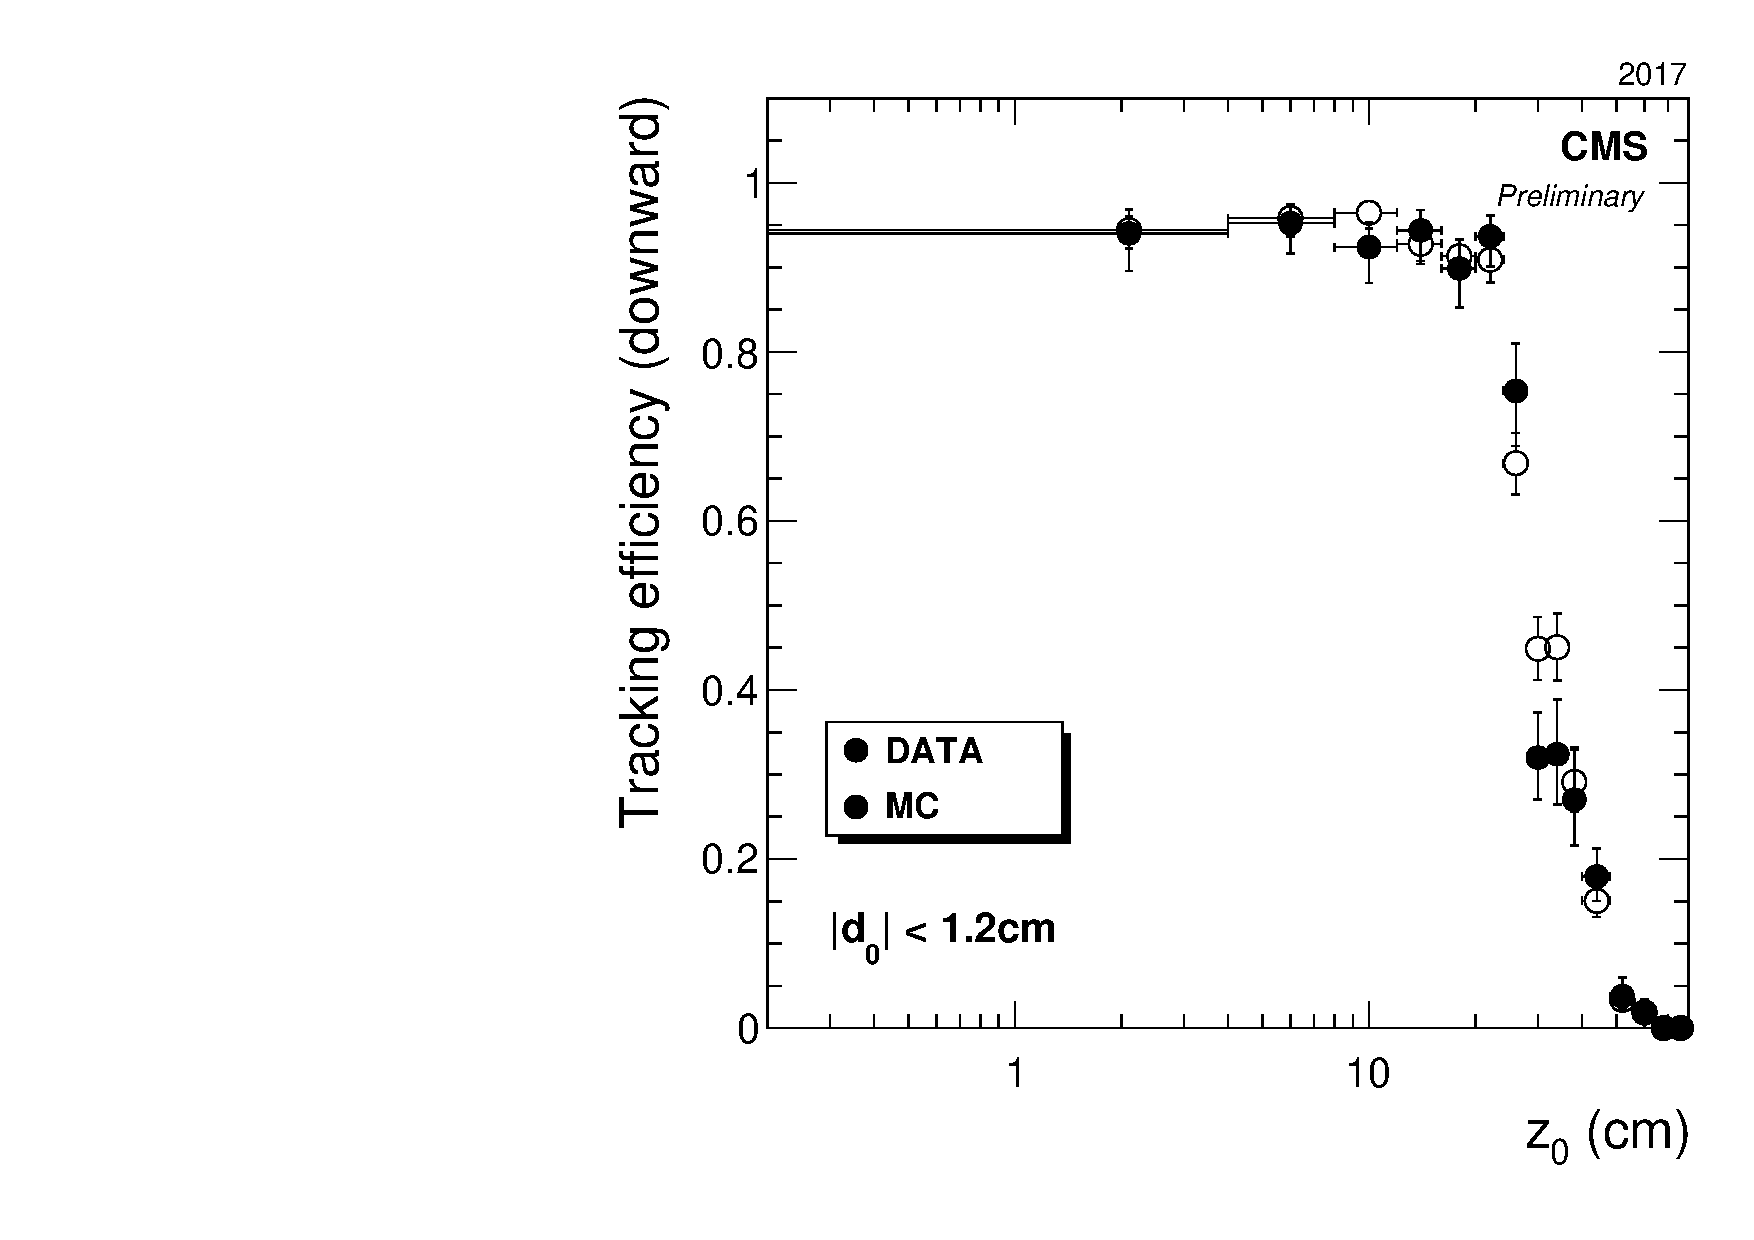
\includegraphics[width=0.4\textwidth]{figures/tracking_eff/2017/Eff0vsZ0.pdf}
\\
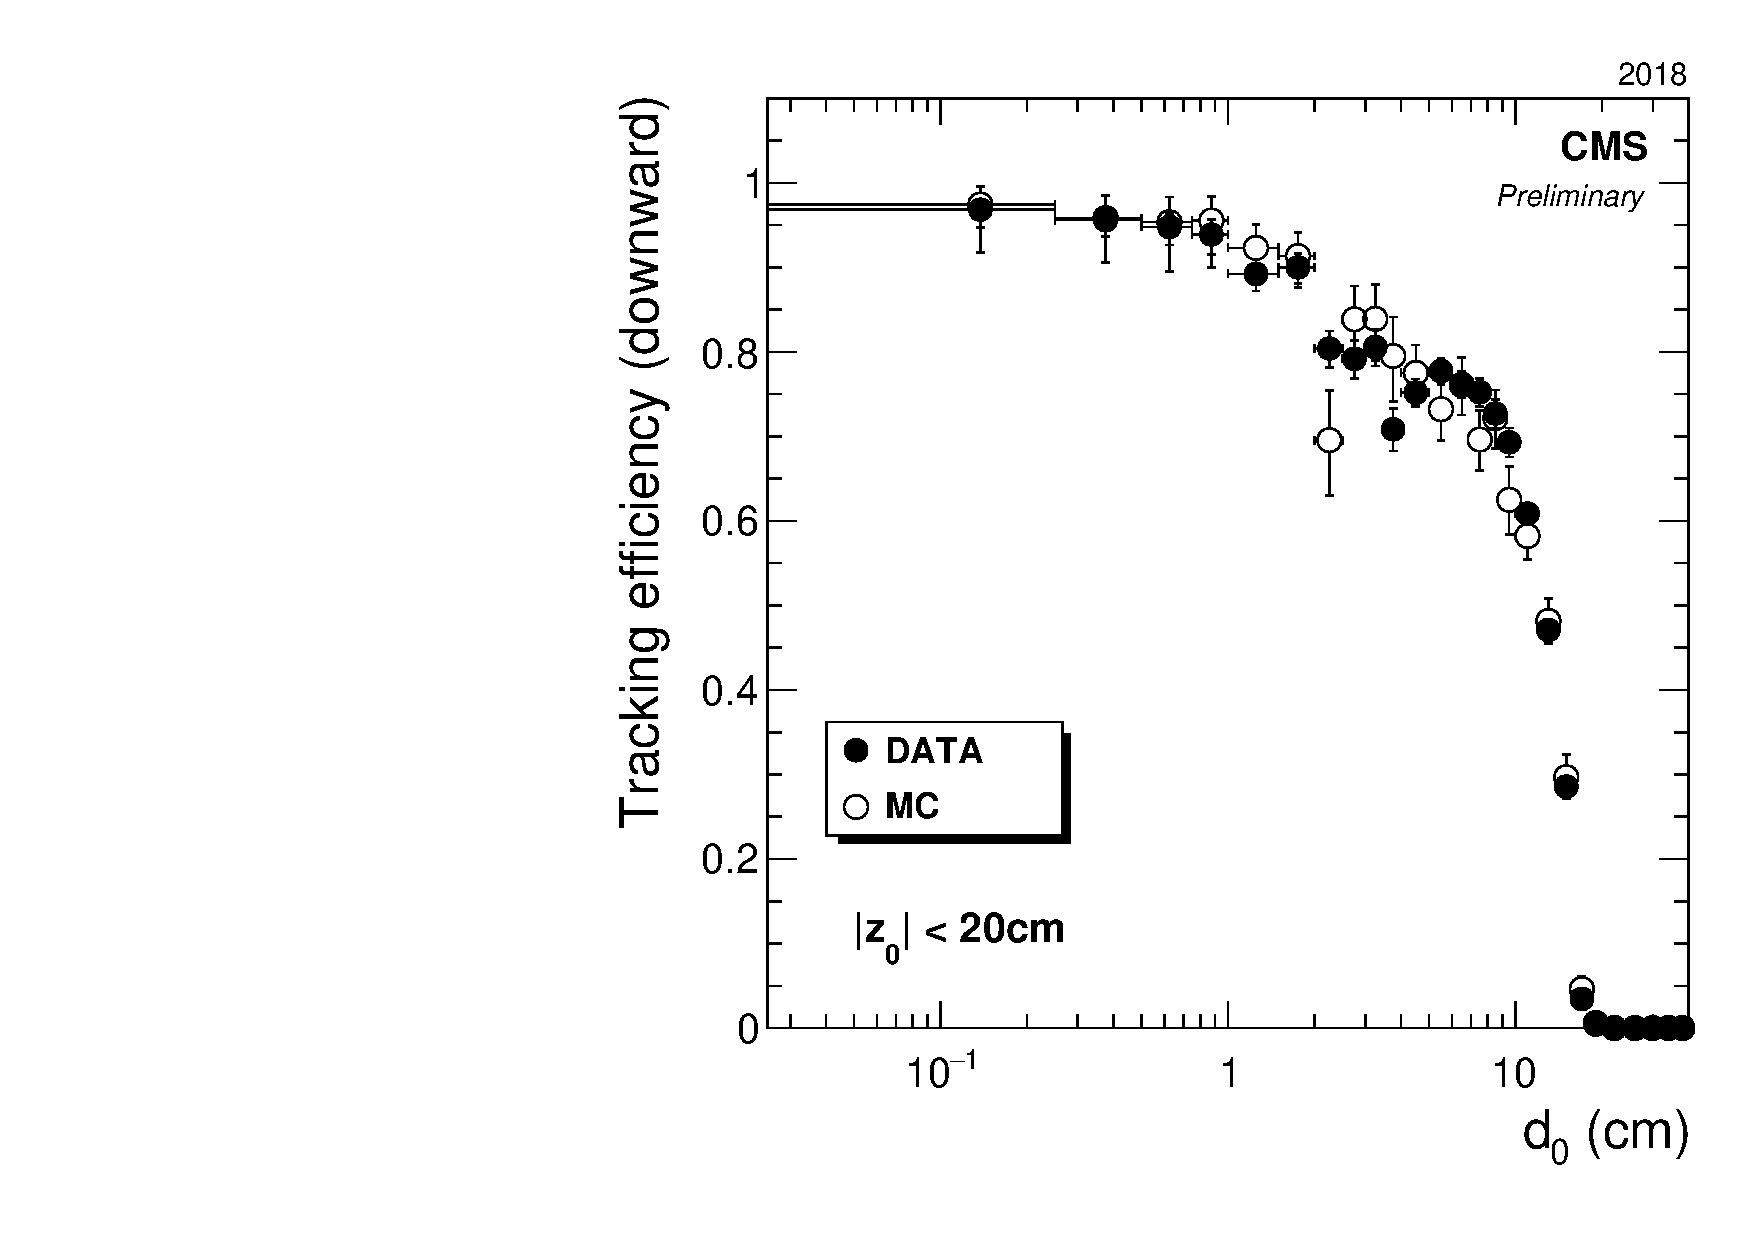
\includegraphics[width=0.4\textwidth]{figures/tracking_eff/2018/Eff0vsD0.pdf}
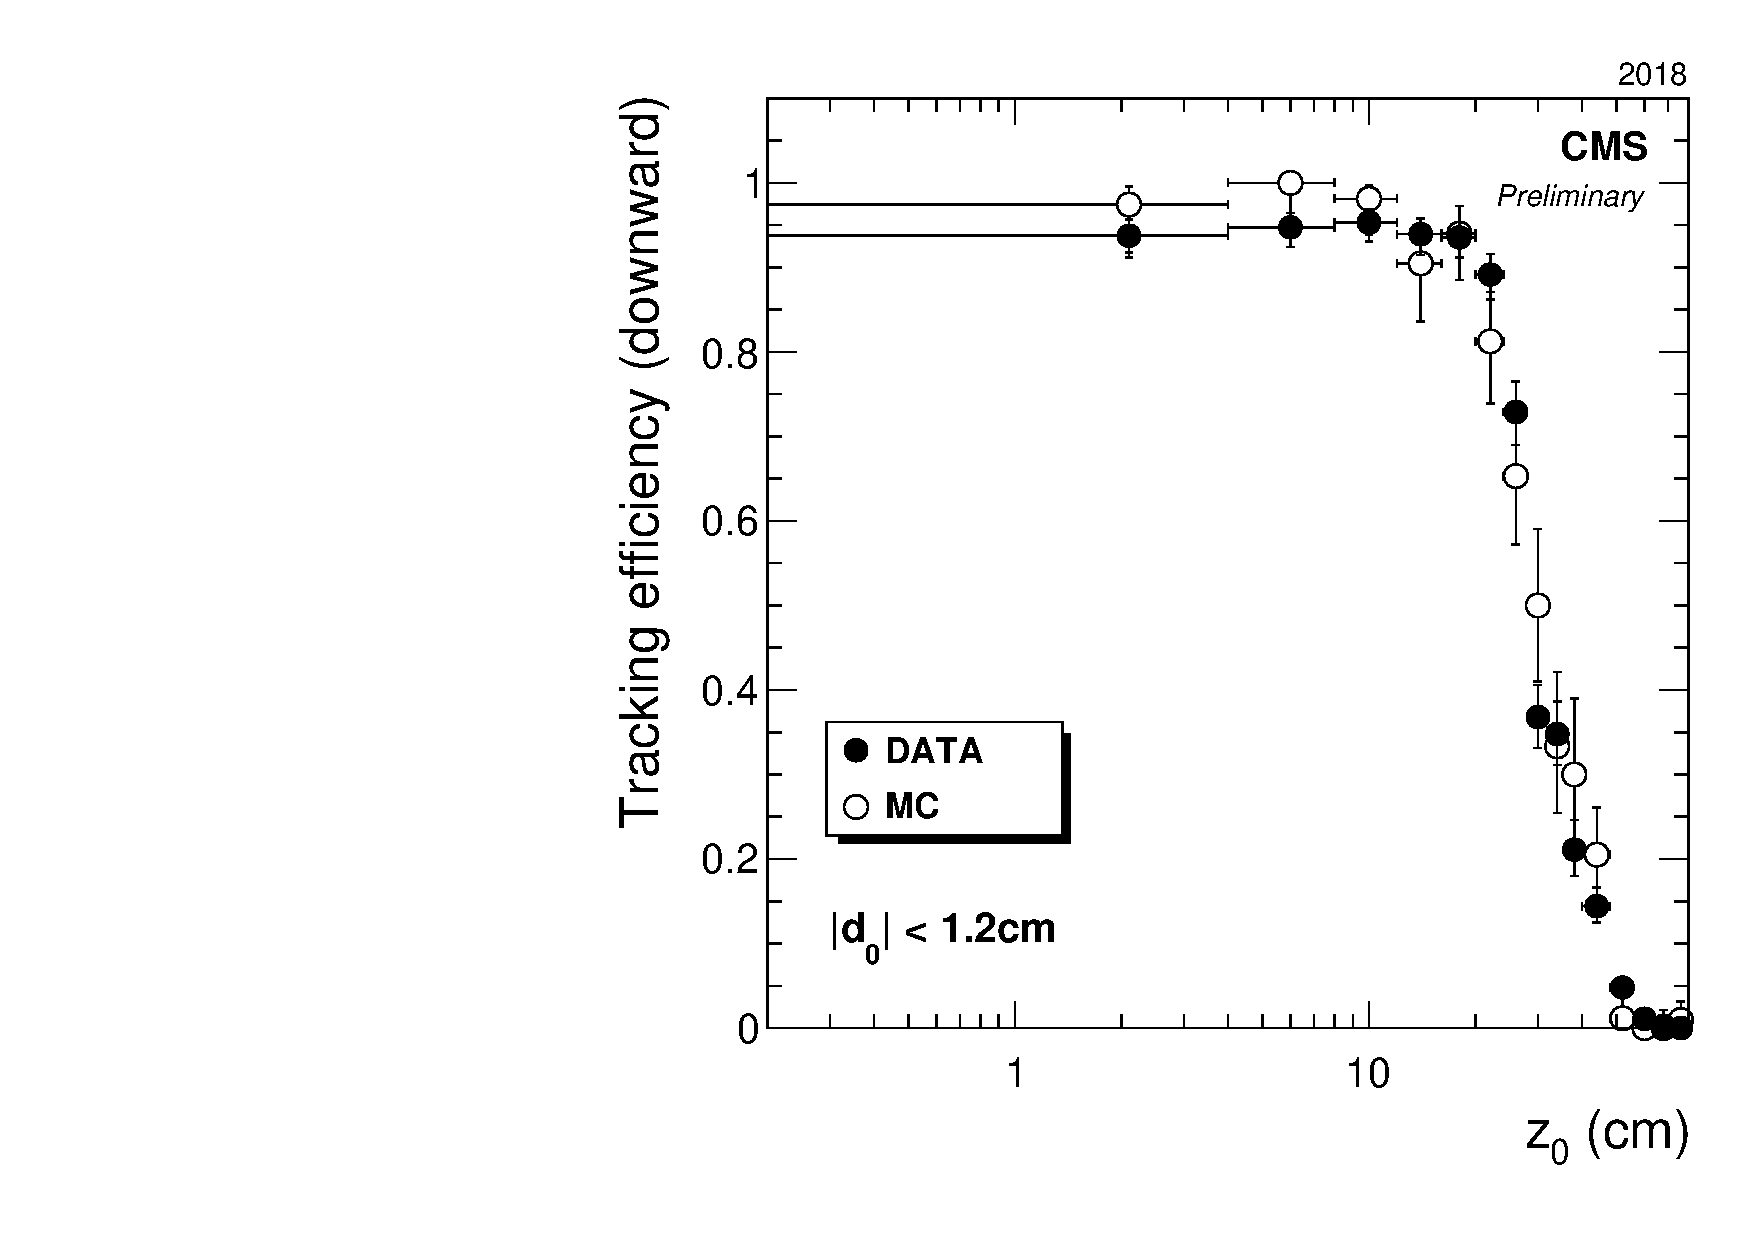
\includegraphics[width=0.4\textwidth]{figures/tracking_eff/2018/Eff0vsZ0.pdf}
\caption{Measured downward tracking efficiency in 2016 (top), 2017 (middle), and 2018 (bottom) versus transverse impact parameter (left) and longitudinal impact parameter (right) in data and simulation. The longitudinal (transverse) impact parameter is constrained to less than \SI{20}{\cm} (\SI{1.2}{\cm}) when plotting against the transverse (longitudinal) impact parameter.}
\label{displaced_trk_eff_vs_d0dz}
\end{figure}

The results of Fig.~\ref{displaced_trk_eff_vs_d0dz} are used to estimate a systematic uncertainty in the simulated signal efficiency arising from the displaced tracking efficiency. A simulated \stoptolb sample with a top squark mass of \SI{1800}{\GeV} and proper decay length $c\tau = \SI{100}{\cm}$ is considered as it produces leptons with the largest impact parameters and therefore represents the most challenging scenario for the displaced track reconstruction. To accommodate the pixel hit requirements, only those events in which both top squarks decay within the volume of the pixel detector are considered. First, the \ad and $\abs{d_z}$ of both leptons in this subset of signal events are noted. Next, a two-dimensional plot of tracking efficiency as a function of \ad and $\abs{d_z}$, $\epsilon(\ad, \az)$, is produced from the cosmic-ray muons in data and simulated cosmic-ray events. Using this plot, the mean efficiency to reconstruct both lepton tracks in the simulated signal events is evaluated as:
\begin{equation}
    \frac{1}{N}\,\sum_i\epsilon(\ad^{(1)}_i, \az^{(1)}_i)\, \epsilon(\ad^{(2)}_i, \az^{(2)}_i)
\end{equation}
where the sum extends over the $N$ events in the signal sample and the superscripts
$(1)$ and $(2)$ denote the two leptons in each event. For each year, the relative systematic uncertainty in the efficiency to reconstruct both lepton tracks is then taken from the ratio of the efficiencies in data and simulation. The resulting efficiencies and systematic uncertainties are listed in Table~\ref{displaced_trk_eff_and_sys}.

\begin{table}
\noindent \centering{}
\topcaption{Mean measured efficiency to reconstruct both lepton tracks in simulated \stoptolb events in data and simulation and the resulting systematic uncertainty. The top squark mass and proper decay length are assumed to be \SI{1800}{\GeV} and \SI{100}{\cm}.}
\label{displaced_trk_eff_and_sys}
\begin{tabular}{l|ccc}
\hline
                         & 2016            & 2017            & 2018\\
\hline
Efficiency in data       & $57.5\pm2.1\%$ & $55.3\pm 1.1\%$ & $56.1\pm 0.7\%$  \\
Efficiency in simulation & $50.3\pm 1.0\%$ & $52.3\pm 0.7\%$ & $57.5\pm 1.1\%$ \\
Systematic uncertainty   & $14.1\pm 4.3\%$ & $ 5.8\pm 2.3\%$ & $ 2.4\pm 2.2\%$ \\
\hline
\end{tabular}
\end{table}